\documentclass{standalone}
\usepackage{tikz}
\usetikzlibrary{shapes, arrows.meta, calc, fit, positioning}

\begin{document}

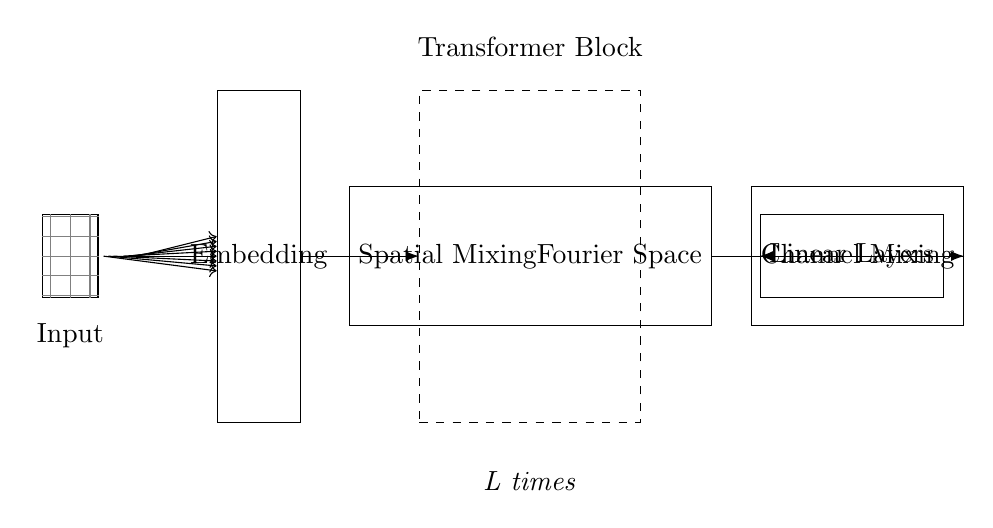
\begin{tikzpicture}[
    block/.style={draw, rectangle, minimum height=3em, minimum width=5em},
    trans_block/.style={draw, dashed, rectangle, minimum height=12em, minimum width=8em},
    embed_block/.style={draw, rectangle, minimum height=12em, minimum width=3em},
    input_block/.style={draw, rectangle, minimum height=3em, minimum width=2em},
    conn/.style={-Latex}
]

% Input block
\node[input_block] (input_block) at (0,0) {};
\draw[step=0.25cm, gray] (input_block.south west) grid (input_block.north east);
\node[below=0.2cm of input_block] {Input};

% Embedding block
\node[embed_block, right=1.5cm of input_block] (embed) {};
\foreach \i in {1,...,8} {
    \draw[->] ($(input_block.east) + (0.125*\i*0.5cm,0)$) -- ($(embed.west) + (0,0.125*\i*0.5cm - 0.25cm)$);
}
\node[align=center] at (embed.center) {Embedding};

% Transformer Block
\node[trans_block, right=1.5cm of embed] (trans) {};
\node[block, minimum height=5em] (spatial) at (trans.center) {Spatial Mixing \\ Fourier Space};
\node[block, right=0.5cm of spatial, minimum height=5em] (channel) {Channel Mixing};
\node[above=0.3cm of trans] {Transformer Block};
\node[below=0.5cm of trans] {\textit{L times}};

% Output of transformer block
\draw[conn] (embed) -- (embed-|trans.west);
\draw[conn] (trans.east -| spatial.east) -- (trans.east -| channel.east);

% Linear layer
\node[block, right=1.5cm of trans] (linear) {Linear Layers};
\draw[conn] (trans.east -| channel.east) -- (linear.west);

\end{tikzpicture}

\end{document}